\documentclass[journal,12pt,twocolumn]{IEEEtran}
\def\inputGnumericTable{}
\usepackage{setspace}
\usepackage{gensymb}
\usepackage{xcolor}
\usepackage{caption}
\singlespacing
\usepackage{siunitx}
\usepackage[cmex10]{amsmath}
\usepackage{mathtools}
\usepackage{hyperref}
\usepackage{amsthm}
\usepackage{mathrsfs}
\usepackage{txfonts}
\usepackage{stfloats}
\usepackage{cite}
\usepackage{cases}
\usepackage{subfig}
\usepackage{longtable}
\usepackage{multirow}
\usepackage{enumitem}
\usepackage{mathtools}
\usepackage{listings}
\usepackage{tikz}
\usetikzlibrary{shapes,arrows,positioning}
\usepackage{circuitikz}
       \usepackage[latin1]{inputenc}
       \usepackage{fullpage}
       \usepackage{color}
       \usepackage{array}
       \usepackage{longtable}
       \usepackage{calc}
       \usepackage{multirow}
       \usepackage{hhline}
       \usepackage{ifthen}
	   \usepackage{setspace}
\let\vec\mathbf
\DeclareMathOperator*{\Res}{Res}
\renewcommand\thesection{\arabic{section}}
\renewcommand\thesubsection{\thesection.\arabic{subsection}}
\renewcommand\thesubsubsection{\thesubsection.\arabic{subsubsection}}

\renewcommand\thesectiondis{\arabic{section}}
\renewcommand\thesubsectiondis{\thesectiondis.\arabic{subsection}}
\renewcommand\thesubsubsectiondis{\thesubsectiondis.\arabic{subsubsection}}
\hyphenation{op-tical net-works semi-conduc-tor}

\lstset{
language=Python,
frame=single, 
breaklines=true,
columns=fullflexible
}
\begin{document}
\theoremstyle{definition}
\newtheorem{theorem}{Theorem}[section]
\newtheorem{problem}{Problem}
\newtheorem{proposition}{Proposition}[section]
\newtheorem{lemma}{Lemma}[section]
\newtheorem{corollary}[theorem]{Corollary}
\newtheorem{example}{Example}[section]
\newtheorem{definition}{Definition}[section]
\newcommand{\BEQA}{\begin{eqnarray}}
        \newcommand{\EEQA}{\end{eqnarray}}
\newcommand{\define}{\stackrel{\triangle}{=}}
\newcommand{\myvec}[1]{\ensuremath{\begin{pmatrix}#1\end{pmatrix}}}
\newcommand{\mydet}[1]{\ensuremath{\begin{vmatrix}#1\end{vmatrix}}}

\bibliographystyle{IEEEtran}
\providecommand{\nCr}[2]{\,^{#1}C_{#2}} % nCr
\providecommand{\nPr}[2]{\,^{#1}P_{#2}} % nPr
\providecommand{\mbf}{\mathbf}
\providecommand{\pr}[1]{\ensuremath{\Pr\left(#1\right)}}
\providecommand{\qfunc}[1]{\ensuremath{Q\left(#1\right)}}
\providecommand{\sbrak}[1]{\ensuremath{{}\left[#1\right]}}
\providecommand{\lsbrak}[1]{\ensuremath{{}\left[#1\right.}}
\providecommand{\rsbrak}[1]{\ensuremath{{}\left.#1\right]}}
\providecommand{\brak}[1]{\ensuremath{\left(#1\right)}}
\providecommand{\lbrak}[1]{\ensuremath{\left(#1\right.}}
\providecommand{\rbrak}[1]{\ensuremath{\left.#1\right)}}
\providecommand{\cbrak}[1]{\ensuremath{\left\{#1\right\}}}
\providecommand{\lcbrak}[1]{\ensuremath{\left\{#1\right.}}
\providecommand{\rcbrak}[1]{\ensuremath{\left.#1\right\}}}
\theoremstyle{remark}
\newtheorem{rem}{Remark}
\newcommand{\sgn}{\mathop{\mathrm{sgn}}}
\newcommand{\rect}{\mathop{\mathrm{rect}}}
\newcommand{\sinc}{\mathop{\mathrm{sinc}}}
\providecommand{\abs}[1]{\left\vert#1\right\vert}
\providecommand{\res}[1]{\Res\displaylimits_{#1}}
\providecommand{\norm}[1]{\lVert#1\rVert}
\providecommand{\mtx}[1]{\mathbf{#1}}
\providecommand{\mean}[1]{E\left[ #1 \right]}
\providecommand{\fourier}{\overset{\mathcal{F}}{ \rightleftharpoons}}
\providecommand{\ztrans}{\overset{\mathcal{Z}}{ \rightleftharpoons}}
\providecommand{\system}[1]{\overset{\mathcal{#1}}{ \longleftrightarrow}}
\newcommand{\solution}{\noindent \textbf{Solution: }}
\providecommand{\dec}[2]{\ensuremath{\overset{#1}{\underset{#2}{\gtrless}}}}
\let\StandardTheFigure\thefigure
\def\putbox#1#2#3{\makebox[0in][l]{\makebox[#1][l]{}\raisebox{\baselineskip}[0in][0in]{\raisebox{#2}[0in][0in]{#3}}}}
\def\rightbox#1{\makebox[0in][r]{#1}}
\def\centbox#1{\makebox[0in]{#1}}
\def\topbox#1{\raisebox{-\baselineskip}[0in][0in]{#1}}
\def\midbox#1{\raisebox{-0.5\baselineskip}[0in][0in]{#1}}

\vspace{3cm}
\title{\LaTeX\ 9.10.6.7}
\author{Lokesh Surana}
\maketitle
\section*{Class 9, Chapter, 10, Exercse 6.7}

Q. AC and BD are chords of a circle which bisect each other. Prove that (i) AC and BD are diameters, (ii) ABCD is a rectangle.

\solution
Let, we have a unit circle with center at origin, i.e. $\vec{O} = \myvec{0\\0}$, and radius $r = 1$.
Let's consider points $A$, $B$, $C$ and $D$ on the circle such that $AC$ and $BD$ are diameter of the circle.
The points on circle that we consider are available in Table \eqref{tab:points}.

\begin{table}[ht!]
%%%%%%%%%%%%%%%%%%%%%%%%%%%%%%%%%%%%%%%%%%%%%%%%%%%%%%%%%%%%%%%%%%%%%%
%%                                                                  %%
%%  This is the header of a LaTeX2e file exported from Gnumeric.    %%
%%                                                                  %%
%%  This file can be compiled as it stands or included in another   %%
%%  LaTeX document. The table is based on the longtable package so  %%
%%  the longtable options (headers, footers...) can be set in the   %%
%%  preamble section below (see PRAMBLE).                           %%
%%                                                                  %%
%%  To include the file in another, the following two lines must be %%
%%  in the including file:                                          %%
%%        \def\inputGnumericTable{}                                 %%
%%  at the beginning of the file and:                               %%
%%        \input{name-of-this-file.tex}                             %%
%%  where the table is to be placed. Note also that the including   %%
%%  file must use the following packages for the table to be        %%
%%  rendered correctly:                                             %%
%%    \usepackage[latin1]{inputenc}                                 %%
%%    \usepackage{color}                                            %%
%%    \usepackage{array}                                            %%
%%    \usepackage{longtable}                                        %%
%%    \usepackage{calc}                                             %%
%%    \usepackage{multirow}                                         %%
%%    \usepackage{hhline}                                           %%
%%    \usepackage{ifthen}                                           %%
%%  optionally (for landscape tables embedded in another document): %%
%%    \usepackage{lscape}                                           %%
%%                                                                  %%
%%%%%%%%%%%%%%%%%%%%%%%%%%%%%%%%%%%%%%%%%%%%%%%%%%%%%%%%%%%%%%%%%%%%%%



%%  This section checks if we are begin input into another file or  %%
%%  the file will be compiled alone. First use a macro taken from   %%
%%  the TeXbook ex 7.7 (suggestion of Han-Wen Nienhuys).            %%
\def\ifundefined#1{\expandafter\ifx\csname#1\endcsname\relax}


%%  Check for the \def token for inputed files. If it is not        %%
%%  defined, the file will be processed as a standalone and the     %%
%%  preamble will be used.                                          %%
\ifundefined{inputGnumericTable}

%%  We must be able to close or not the document at the end.        %%
	\def\gnumericTableEnd{\end{document}}


%%%%%%%%%%%%%%%%%%%%%%%%%%%%%%%%%%%%%%%%%%%%%%%%%%%%%%%%%%%%%%%%%%%%%%
%%                                                                  %%
%%  This is the PREAMBLE. Change these values to get the right      %%
%%  paper size and other niceties.                                  %%
%%                                                                  %%
%%%%%%%%%%%%%%%%%%%%%%%%%%%%%%%%%%%%%%%%%%%%%%%%%%%%%%%%%%%%%%%%%%%%%%

	\documentclass[12pt%
			  %,landscape%
                    ]{report}
       \usepackage[latin1]{inputenc}
       \usepackage{fullpage}
       \usepackage{color}
       \usepackage{array}
       \usepackage{longtable}
       \usepackage{calc}
       \usepackage{multirow}
       \usepackage{hhline}
       \usepackage{ifthen}

\begin{document}


%%  End of the preamble for the standalone. The next section is for %%
%%  documents which are included into other LaTeX2e files.          %%
\else

%%  We are not a stand alone document. For a regular table, we will %%
%%  have no preamble and only define the closing to mean nothing.   %%
\def\gnumericTableEnd{}

%%  If we want landscape mode in an embedded document, comment out  %%
%%  the line above and uncomment the two below. The table will      %%
%%  begin on a new page and run in landscape mode.                  %%
%       \def\gnumericTableEnd{\end{landscape}}
%       \begin{landscape}


%%  End of the else clause for this file being \input.              %%
\fi

%%%%%%%%%%%%%%%%%%%%%%%%%%%%%%%%%%%%%%%%%%%%%%%%%%%%%%%%%%%%%%%%%%%%%%
%%                                                                  %%
%%  The rest is the gnumeric table, except for the closing          %%
%%  statement. Changes below will alter the table's appearance.     %%
%%                                                                  %%
%%%%%%%%%%%%%%%%%%%%%%%%%%%%%%%%%%%%%%%%%%%%%%%%%%%%%%%%%%%%%%%%%%%%%%

\providecommand{\gnumericmathit}[1]{#1}
%%  Uncomment the next line if you would like your numbers to be in %%
%%  italics if they are italizised in the gnumeric table.           %%
%\renewcommand{\gnumericmathit}[1]{\mathit{#1}}
\providecommand{\gnumericPB}[1]%
{\let\gnumericTemp=\\#1\let\\=\gnumericTemp\hspace{0pt}}
\ifundefined{gnumericTableWidthDefined}
\newlength{\gnumericTableWidth}
\newlength{\gnumericTableWidthComplete}
\newlength{\gnumericMultiRowLength}
\global\def\gnumericTableWidthDefined{}
\fi
%% The following setting protects this code from babel shorthands.  %%
\ifthenelse{\isundefined{\languageshorthands}}{}{\languageshorthands{english}}
%%  The default table format retains the relative column widths of  %%
%%  gnumeric. They can easily be changed to c, r or l. In that case %%
%%  you may want to comment out the next line and uncomment the one %%
%%  thereafter                                                      %%
\providecommand\gnumbox{\makebox[0pt]}
%%\providecommand\gnumbox[1][]{\makebox}

%% to adjust positions in multirow situations                       %%
\setlength{\bigstrutjot}{\jot}
\setlength{\extrarowheight}{\doublerulesep}

%%  The \setlongtables command keeps column widths the same across  %%
%%  pages. Simply comment out next line for varying column widths.  %%
\setlongtables

\setlength\gnumericTableWidth{%
       53pt+%
       171pt+%
       53pt+%
       0pt}
\def\gumericNumCols{3}
\setlength\gnumericTableWidthComplete{\gnumericTableWidth+%
       \tabcolsep*\gumericNumCols*2+\arrayrulewidth*\gumericNumCols}
\ifthenelse{\lengthtest{\gnumericTableWidthComplete > \linewidth}}%
{\def\gnumericScale{1*\ratio{\linewidth-%
                     \tabcolsep*\gumericNumCols*2-%
                     \arrayrulewidth*\gumericNumCols}%
              {\gnumericTableWidth}}}%
{\def\gnumericScale{1}}

%%%%%%%%%%%%%%%%%%%%%%%%%%%%%%%%%%%%%%%%%%%%%%%%%%%%%%%%%%%%%%%%%%%%%%
%%                                                                  %%
%% The following are the widths of the various columns. We are      %%
%% defining them here because then they are easier to change.       %%
%% Depending on the cell formats we may use them more than once.    %%
%%                                                                  %%
%%%%%%%%%%%%%%%%%%%%%%%%%%%%%%%%%%%%%%%%%%%%%%%%%%%%%%%%%%%%%%%%%%%%%%

\ifthenelse{\isundefined{\gnumericColA}}{\newlength{\gnumericColA}}{}\settowidth{\gnumericColA}{\begin{tabular}{@{}p{53pt*\gnumericScale}@{}}x\end{tabular}}
\ifthenelse{\isundefined{\gnumericColB}}{\newlength{\gnumericColB}}{}\settowidth{\gnumericColB}{\begin{tabular}{@{}p{171pt*\gnumericScale}@{}}x\end{tabular}}
\ifthenelse{\isundefined{\gnumericColC}}{\newlength{\gnumericColC}}{}\settowidth{\gnumericColC}{\begin{tabular}{@{}p{53pt*\gnumericScale}@{}}x\end{tabular}}

\begin{tabular}[c]{%
              b{\gnumericColA}%
              b{\gnumericColB}%
              b{\gnumericColC}%
       }

       %%%%%%%%%%%%%%%%%%%%%%%%%%%%%%%%%%%%%%%%%%%%%%%%%%%%%%%%%%%%%%%%%%%%%%
       %%  The longtable options. (Caption, headers... see Goosens, p.124) %%
       %	\caption{The Table Caption.}             \\	%
       % \hline	% Across the top of the table.
       %%  The rest of these options are table rows which are placed on    %%
       %%  the first, last or every page. Use \multicolumn if you want.    %%

       %%  Header for the first page.                                      %%
       %	\multicolumn{3}{c}{The First Header} \\ \hline 
       %	\multicolumn{1}{c}{colTag}	%Column 1
       %	&\multicolumn{1}{c}{colTag}	%Column 2
       %	&\multicolumn{1}{c}{colTag}	\\ \hline %Last column
       %	\endfirsthead

       %%  The running header definition.                                  %%
       %	\hline
       %	\multicolumn{3}{l}{\ldots\small\slshape continued} \\ \hline
       %	\multicolumn{1}{c}{colTag}	%Column 1
       %	&\multicolumn{1}{c}{colTag}	%Column 2
       %	&\multicolumn{1}{c}{colTag}	\\ \hline %Last column
       %	\endhead

       %%  The running footer definition.                                  %%
       %	\hline
       %	\multicolumn{3}{r}{\small\slshape continued\ldots} \\
       %	\endfoot

       %%  The ending footer definition.                                   %%
       %	\multicolumn{3}{c}{That's all folks} \\ \hline 
       %	\endlastfoot
       %%%%%%%%%%%%%%%%%%%%%%%%%%%%%%%%%%%%%%%%%%%%%%%%%%%%%%%%%%%%%%%%%%%%%%

       \hhline{|-|-|-}
       \multicolumn{1}{|p{\gnumericColA}|}%
       {\gnumericPB{\raggedright}\gnumbox[l]{$O$}}
        & \multicolumn{1}{p{\gnumericColB}|} %
       {\gnumericPB{\raggedright}\gnumbox[l]{Lowest point of cable}}
        & \multicolumn{1}{p{\gnumericColC}|} %
       {\gnumericPB{\raggedright}\gnumbox[l]{\myvec{0\\0}}}
       \\
       \hhline{|-|-|-|}
       \multicolumn{1}{|p{\gnumericColA}|}%
       {\gnumericPB{\raggedright}\gnumbox[l]{$AB$}}
        & \multicolumn{1}{p{\gnumericColB}|} %
       {\gnumericPB{\raggedright}\gnumbox[l]{Length of the cable}}
        & \multicolumn{1}{p{\gnumericColC}|} %
       {\gnumericPB{\raggedright}\gnumbox[l]{100 m}}
       \\
       \hhline{|-|-|-|}
       \multicolumn{1}{|p{\gnumericColA}|}%
       {\gnumericPB{\raggedright}\gnumbox[l]{$OC$}}
        & \multicolumn{1}{p{\gnumericColB}|} %
       {\gnumericPB{\raggedright}\gnumbox[l]{Length of shortest wire }}
        & \multicolumn{1}{p{\gnumericColC}|} %
       {\gnumericPB{\raggedright}\gnumbox[l]{6 m}}
       \\
       \hhline{|-|-|-|}
       \multicolumn{1}{|p{\gnumericColA}|}%
       {\gnumericPB{\raggedright}\gnumbox[l]{$C_1A$}}
        & \multicolumn{1}{p{\gnumericColB}|} %
       {\gnumericPB{\raggedright}\gnumbox[l]{Length of longest wire }}
        & \multicolumn{1}{p{\gnumericColC}|} %
       {\gnumericPB{\raggedright}\gnumbox[l]{30 m}}
       \\
       \hhline{|-|-|-|}
\end{tabular}

\ifthenelse{\isundefined{\languageshorthands}}{}{\languageshorthands{\languagename}}
\gnumericTableEnd

\caption{}
\label{tab:points}
\end{table}

\begin{enumerate}
    \item $AC$ and $BD$ are diameters of the circle. Let's check if they bisect each other,
    \begin{align}
        \vec{A} + \vec{C} &= \myvec{1 \\ 0} + \myvec{-1 \\ 0}\\
        \label{eq:1} &= \myvec{0 \\ 0} \\
        \vec{B} + \vec{D} &= \myvec{1 \\ 0} + \myvec{-1 \\ 0}\\
        \label{eq:2} &= \myvec{0 \\ 0}
    \end{align}
    From equation \eqref{eq:1} and \eqref{eq:2} $AC$ and $BD$ bisect each other.
    Hence, we can say that if two chords bisect each other then they are diameters.

    \item Let's check if $ABCD$ is a rectangle.
    The sides of a rectangle are parallel to each other. Let's check if $AB$ and $BC$ are parallel to each other.
    \begin{align}
        \vec{A} - \vec{B} &= \myvec{1 \\ 0} - \myvec{0 \\ 1}\\
        \label{eq:4} &= \myvec{1 \\ -1} \\
        \vec{D} - \vec{C} &= \myvec{0\\ -1} - \myvec{-1 \\ 0}\\
        \label{eq:5} &= \myvec{1 \\ -1} 
    \end{align}
    From equation \eqref{eq:4} and \eqref{eq:5}, $AB$ and $DC$ are parallel to each other.
    $\implies ABCD$ is a parallelogram.

    Now let's check if its a rectangle.
    Let's check the angle between adjacent sides of this quadrilateral, i.e. $AB$ and $BC$.

    \begin{align}
        \vec{A} - \vec{B} &= \myvec{1 \\ 0} - \myvec{0 \\ 1} \\
        &= \myvec{1 \\ -1} \\
        \vec{B} - \vec{C} &= \myvec{0 \\ 1} - \myvec{-1 \\ 0} \\
        &= \myvec{1 \\ 1} \\
        \label{eq:6} \brak{\vec{A} - \vec{B}}^\top \brak{\vec{B} - \vec{C}} &=  \myvec{1 & -1} \myvec{1 \\ 1} \\
        &= 0
    \end{align}

    From equation \eqref{eq:6}, we can say that the angle between $AB$ and $BC$ is $90\degree$.
    Hence, the quadrilateral $ABCD$ is a rectangle.
\end{enumerate}

\begin{figure}[!htb]
    \centering
    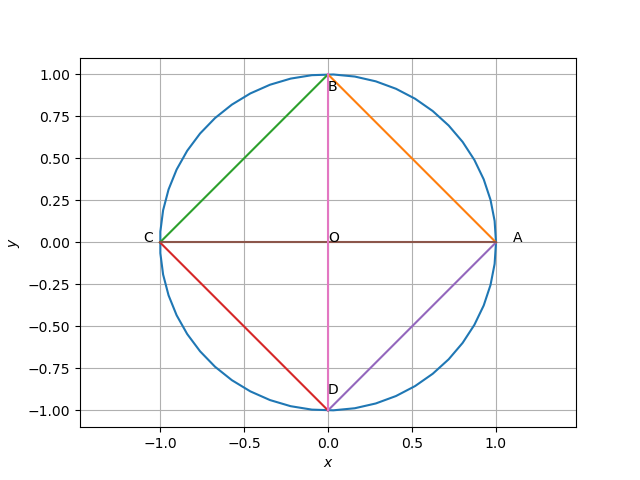
\includegraphics[width=\columnwidth]{figs/circle.png}
    \caption{circle}
    \label{fig:circle}
\end{figure}

\end{document}